\graphicspath{{Figures/}}

\title{\fontsize{33}{45}{\huge Pattern Classification (EET 3035)\newline \vspace{8pt} \Large Lecture 03\vspace{-1.1cm}}}
\author{\vspace{-0.4cm}\\\normalsize{\bf Dr. Kundan Kumar}\\ PhD (IIT Kharagpur)\\
Associate Professor\\Department of ECE}
% - Give the names in the same order as the appear in the paper.
% - Use the \inst{?} command only if the authors have different
%   affiliation.

\institute[Indian Institute of Technology Kharagpur] % (optional, but mostly needed)
{
\includegraphics[height=.17\textheight]{SOAlogo.png}\\
 Faculty of Engineering (ITER)\\ S`O'A Deemed to be University, Bhubaneswar, India-751030\\
 \copyright\  2020 Kundan Kumar, All Rights Reserved\\
  \vspace{-1.1cm}}
% - Use the \inst command only if there are several affiliations.
% - Keep it simple, no one is interested in your street address.
\date{}
% To remove page number from a perticular slide
{
\setbeamertemplate{logo}{}
\makeatletter
\setbeamertemplate{footline}{
        \leavevmode%
  
  % First line.
  \hbox{%
  \begin{beamercolorbox}[wd=.2\paperwidth,ht=\beamer@decolines@lineup,dp=0pt]{}%
  \end{beamercolorbox}%
  \begin{beamercolorbox}[wd=.8\paperwidth,ht=\beamer@decolines@lineup,dp=0pt]{lineup}%
  \end{beamercolorbox}%
  } %
  % Second line.
  \hbox{%
  \begin{beamercolorbox}[wd=\paperwidth,ht=\beamer@decolines@linemid,dp=0pt]{linemid}%
  \end{beamercolorbox}%
  } %
  % Third line.
  \hbox{%
  \begin{beamercolorbox}[wd=.1\paperwidth,ht=\beamer@decolines@linebottom,dp=0pt]{}%
  \end{beamercolorbox}%
  \begin{beamercolorbox}[wd=.9\paperwidth,ht=\beamer@decolines@linebottom,dp=0pt]{linebottom}%
  \end{beamercolorbox}%
  }%
        }
\makeatother
\begin{frame}
\titlepage
\end{frame}
}


\section{Bayesian Decision Theory}
\subsection{}
\begin{frame}{}
\begin{variableblock}{\centering \Large \textbf{\vspace{4pt}\newline Bayesian Decision Theory\vspace{4pt}}}{bg=slidecolor,fg=white}{bg=slidecolor,fg=white}
\end{variableblock}
\end{frame}

\begin{frame}{Bayesian Decision Theory}
\begin{itemize}
\setlength{\itemsep}{8pt}
\item \textit{\color{mycolor1}Bayesian Decision Theory} is a fundamental statistical
approach that quantifies the trade-offs between various
decisions using probabilities and costs that accompany
such decisions.\nocite{duda2012pattern}
\item First, we will assume that all probabilities are known.
\item Then, we will study the cases where the probabilistic
structure is not completely known.
\end{itemize}
\end{frame}

\begin{frame}{Fish Sorting Example Revisited}
\begin{itemize}
\item \textit{\color{mycolor1}State of nature} (class) is a random variable.
\item Define $\omega$ as the type of fish we observe (state of nature, class) where
\begin{itemize}
\item $\omega=\omega_1$ for sea bass,
\item $\omega=\omega_2$ for salmon.
\item $P(\omega_1)$ is the \textit{\color{mycolor1}a priori probability} that the next fish is a sea bass.
\item $P(\omega_2)$ is the \textit{a priori probability} that the next fish is a salman.
%\item $P(\omega_1)+P(\omega_2)=1$, if no other types of fish are relevant.
%\item e.g., prior knowledge of how likely is to get a sea bass or a salmon
\end{itemize}
\end{itemize}
\end{frame}

\begin{frame}{Prior Probabilities}
\begin{itemize}
\setlength{\itemsep}{12pt}
\item Prior probabilities reflect our knowledge of how likely each type of fish will appear before we actually see it.
\item How can we choose $P(\omega_1)$ and $P(\omega_2)$?
\begin{itemize}
\item Set $P(\omega_1)=P(\omega_2)$ if they are equiprobable ({\color{mycolor1}uniform priors}).
\item May use different values depending on the fishing area, time of the year, etc.
\end{itemize}
\item Assume there are no other types of fish
\[\boxed{P(\omega_1)+P(\omega_2)=1}\]
(exclusivity and exhaustivity)
\end{itemize}
\end{frame}

\begin{frame}{Making a Decision}
\begin{itemize}
%\setlength{\itemsep}{12pt}
\item How can we make a decision with only the prior
information? (\textit{\color{mycolor1}Decision rule})
\onslide<2->{\begin{equation}
\boxed{{\sf Decide}~~~~\left\{ {\begin{array}{*{20}{c}}
{{\omega_1}}&{{\sf if}~P({\omega_1}) > P({\omega_2})}\\
{{\omega_2}}&{\sf otherwise~~~~~~~}
\end{array}} \right.\nonumber}
\end{equation}}
\onslide<3->{\item What is the \textit{\color{mycolor1}probability of error} for this decision?}
\onslide<4->{\begin{equation}
\boxed{P(error)=\min\{P(\omega_1),P(\omega_2)\}\nonumber}
\end{equation}}
\onslide<5->{\item Don't you feel that there is some problem in making a decision?}
\end{itemize}
\end{frame}

\begin{frame}{Class-Conditional Probabilities}
\begin{itemize}
\item Let's try to improve the decision using the lightness
measurement $x$.
\item Let $x$ be a continuous random variable.
\item Probability density function $p(x)$ (\textit{\color{mycolor1}evidence})
\begin{itemize}
\item how frequently we will measure a pattern with feature value $x$ (e.g., $x$ corresponds to lightness)
\end{itemize}
\item Define $p(x|\omega_j )$ as the \textit{\color{mycolor1}class-conditional probability density}
\begin{itemize}
\item how frequently we will measure a pattern with feature value $x$ given that pattern belongs to class $\omega_j$
\end{itemize}
\item $p(x|\omega_1)$ and $p(x|\omega_2)$ describe the difference in lightness
between populations of sea bass and salmon.
\end{itemize}
\end{frame}
%
%%\begin{frame}[allowframebreaks]{Terminology}
%%\begin{itemize}
%%\item \textbf{State of nature:} $w$ (class label)
%%\begin{itemize}
%%\item e.g., $\omega_1$ for sea bass, $\omega_2$ for salmon
%%\end{itemize}
%%\item Probabilities $P(\omega_1)$ and $P(\omega_2)$ \textbf{(Priors)}
%%\begin{itemize}
%%\item $P(\omega_1)+P(\omega_2)=1$, if no other types of fish are relevant.
%%\item e.g., prior knowledge of how likely is to get a sea bass or a salmon
%%\end{itemize}
%%\item Probability density function $p(x)$ \textbf{(evidence)}
%%\begin{itemize}
%%\item e.g., how frequently we will measure a pattern with feature value $x$ (e.g., $x$ corresponds to lightness)
%%\end{itemize}
%%\item \textbf{Decision rule}: Decide $\omega_1$ if $P(\omega_1)>P(\omega_2)$; otherwise decide $\omega_2$
%%\end{itemize}
%%\end{frame}

\begin{frame}{Class-Conditional Probabilities}
\begin{figure}
\includegraphics[scale=0.65]{Bayes01}
\caption{Hypothetical class-conditional probability density functions (lightness) for salmon/sea-bass}
\end{figure}
\end{frame}

\begin{frame}{Posterior Probabilities}
\begin{itemize}
\item Suppose we know $P(\omega_j)$ and $p(x|\omega_j)$ for $j=1,2$ and measure the lightness of a fish as the value $x$.
\item Define $P(\omega_j|x)$ as the a \textit{\color{mycolor1}posterior probability} (probability of the state of nature being $\omega_j$ given the measurement of feature value $x$)
\item We can use the \textit{\color{mycolor1}Bayes formula} to convert the prior probability to the posterior probability
\begin{equation}
\boxed{P({\omega_j}|x) = \frac{{p(x|{\omega_j})P({\omega_j})}}{{p(x)}} = \frac{{likelihood \times prior}}{{evidence}}\nonumber}
\end{equation}
where $p(x) = \sum\limits_{j = 1}^2 {p(x|{\omega_j})P({\omega_j})} $
\end{itemize}
\end{frame}

\begin{frame}{Posterior Probabilities}
\begin{figure}
\includegraphics[scale=0.68]{Bayes33}
\caption{ Posterior probabilities for the particular priors $P(\omega_1) = 2/3$ and $P(\omega_2 ) =1/3$ for the class-conditional probability densities. Thus in this case,
given that a pattern is measured to have feature value $x = 14$, the probability it is in category $\omega_2$ is roughly 0.08, and that it is in $\omega_1$ is 0.92. At every $x$, the posteriors
sum to 1.0.}
\end{figure}
\end{frame}

\begin{frame}{Making a Decision}
\begin{itemize}
\item $p(x|\omega_j)$ is called the \textit{\color{mycolor1}likelihood} and $p(x)$ is called the \textit{\color{mycolor1}evidence}.
\item How can we make a decision after observing the value of $x$?
\begin{equation}
\boxed{{\sf Decide}~~~~\left\{ {\begin{array}{*{20}{c}}
{{\omega_1}}&{{\sf if}~P({\omega_1}|x) > P({\omega_2}|x)}\\
{{\omega_2}}&{\sf otherwise~~~~~~~~~~~~~~~~~~}
\end{array}} \right.\nonumber}
\end{equation}
\item Rewriting the rule gives
\begin{equation}
\boxed{{\sf Decide}~~~~\left\{ {\begin{array}{*{20}{c}}
{{\omega_1}}&{{\sf if}~{p(x|\omega_1)P(\omega_1)}>{p(x|\omega_2)P(\omega_2)}}\\
{{\omega_2}}&{\sf otherwise~~~~~~~~~~~~}
\end{array}} \right.\nonumber}
\end{equation}
\item Note that, at every $x$, $P(\omega_1|x)+P(\omega_2|x)=1$
\end{itemize}
\end{frame}
%
%%\begin{frame}{Posterior Probabilities}
%%\begin{itemize}
%%\item Conditional probability $P(\omega_j/x)$ (Posterior)
%%\begin{itemize}
%%\item e.g., the probability that the fish belongs to class $\omega_j$ given feature $x$
%%\end{itemize}
%%\item Ultimately, we are interested in computing $P(\omega_j/x)$ for each class $\omega_j$.
%%\end{itemize}
%%\end{frame}
%
%%\begin{frame}{Decision rule using Prior probabilities only}
%%\fbox{\begin{minipage}
%%{\textwidth}
%%\centering
%%Decide $\omega_1$ if $P(\omega_1)>P(\omega_2)$; otherwise decide $\omega_2$
%%\end{minipage}}
%%\[P(error) = \left\{ {\begin{array}{*{20}{c}}
%%{P({\omega_1})\text{ if we decide }{\omega_2}}\\
%%{P({\omega_2})\text{ if we decide }{\omega_1}}
%%\end{array}} \right.\]
%%\hspace{49pt}or $P(error) = min[P({\omega_1}),P({\omega_2})]$
%%\vspace{12pt}
%%\begin{itemize}
%%\item Favours the most likely class.
%%\item This rule will be making the same decision all times.
%%\begin{itemize}
%%\item i.e., optimum if no other information is available.
%%\end{itemize}
%%\end{itemize}
%%\end{frame}
%
%%\begin{frame}{Decision rule using Conditional Probabilities}
%%\begin{itemize}
%%\item Bayes' rule:
%%\fbox{\begin{minipage}
%%{0.8\textwidth}
%%\centering
%%\begin{equation}
%%P({\omega_j}/x) = \frac{{p(x/{\omega_j})P({\omega_j})}}{{p(x)}} = \frac{{likelihood \times prior}}{{evidence}}
%%\end{equation}
%%\end{minipage}}\\
%%where $p(x) = \sum\limits_{j = 1}^2 {p(x/{\omega_j})P({\omega_j})} $
%%\item Decide $\omega_1$ if $P(\omega_1/x)>P(\omega_2/x)$; otherwise decide $\omega_2$
%%\item Decide $\omega_1$ if $p(x/\omega_1)P(\omega_1)>p(x/\omega_2)P(\omega_2)$; otherwise decide $\omega_2$
%%\item Decide $\omega_1$ if $p(x/\omega_1)/p(x/\omega_2)>P(\omega_2)/P(\omega_1)$; otherwise decide $\omega_2$
%%\end{itemize}
%%\end{frame}

\begin{frame}{Probability of Error}
\begin{itemize}
\item What is the probability of error for this decision?
\begin{equation}
\boxed{P(error|x)=\left\{ {\begin{array}{*{20}{c}}
{P(\omega_1|x)}&{{\sf if~we~decide~}\omega_2}\\
{P(\omega_2|x)}&{{\sf if~we~decide~}\omega_1}
\end{array}} \right.\nonumber}
\end{equation}
\item What is the average probability of error?
\[P(error)=\int_{-\infty}^{\infty}P(error,x)dx=\int_{-\infty}^{\infty}P(error|x)p(x)dx\]
\item Bayes decision rule minimizes this error because
\[P(error|x)=\min\{P(\omega_1|x),P(\omega_2|x)\}\]
\end{itemize}
\end{frame}

\begin{frame}{Generalization of the preceding ideas}
\textbf{\color{mycolor1}Generalization of Bayes decision rule}
\begin{itemize}
\setlength{\itemsep}{8pt}
\item Use of more than one feature, e.g., $\{x_1,~x_2,\ldots ,x_d\}$
\item Use more than two states of nature, e.g., $\{\omega_1,~\omega_2,\ldots ,\omega_c\}$
\item Allowing actions and not only decide on the state of nature
\begin{itemize}
\item take an action from the set of predefined actions $\{\alpha_1,\alpha_2,\ldots,\alpha_a\}$.
\end{itemize}
\item Introduce a loss of function which is more general than the probability of error
\begin{itemize}
\item Loss incurred $\lambda (\alpha_i|\omega_j)$ for taking action $\alpha_i$ while the true state of nature is $\omega_j$.
\end{itemize}
\end{itemize}
\end{frame}

\begin{frame}{Generalization of the preceding ideas}
\begin{itemize}
\setlength{\itemsep}{12pt}
\item Allowing the use of more than one feature merely requires replacing the scalar $x$ by the feature vector ${\rm x}$, where ${\rm x}$ is in a \textit{\color{mycolor1}$d$-dimensional Euclidean space}, $\mathbb{R}^d$, called the \textit{\color{mycolor1}feature space}.
\item Allowing actions other than classification primarily allows the \textit{\color{mycolor1}possibility of rejection} -- that is, of refusing to make a decision in close cases.
\item The \textit{\color{mycolor1}loss function} states exactly how costly each action is, and is used to convert a probability determination into a decision.
\end{itemize}
\end{frame}

\begin{frame}{Bayesian Decision Theory -- Continuous Features}
\begin{itemize}
\item Let $\{\omega_1,\omega_2,\ldots,\omega_c\}$ be the finite set of $c$ states of nature (or ``\textit{\color{mycolor1}classes}'', ``\textit{\color{mycolor1}categories}'')
\item Let $\{\alpha_1,\alpha_2,\ldots,\alpha_a\}$ be the finite set of `$a$' possible \textit{\color{mycolor1}actions}.
\item Let $\lambda(\alpha_i|\omega_j)$ be the \textit{\color{mycolor1}loss} incurred for taking action $\alpha_i$ when the state of nature is $\omega_j$.
\item Let ${\rm x}$ be the $d$-component vector-valued random variable called the \textit{\color{mycolor1}feature vector}.
%\item Suppose that we observe a particular ${\rm x}$ and that we contemplate taking action $\alpha_i$, So if the true state of nature is $\omega_j$ then loss incurred $\lambda(\alpha_i/\omega_j)$.
%\item Total loss associated with taking action $\alpha_i$ is
%\begin{figure}
%\includegraphics[scale=1]{Ch0215}
%\end{figure}
\end{itemize}
\end{frame}

\begin{frame}{Bayesian Decision Theory -- Continuous Features}
\begin{itemize}
\setlength{\itemsep}{4pt}
\item $p({\rm x}|\omega_j)$ is the class-conditional probability density function.
\item $P(\omega_j)$ is the prior probability that nature is in state $\omega_j$.
\item The posterior probability can be computed as
\[\boxed{P(\omega_j|{\rm x})=\frac{p({\rm x}|\omega_j)P(\omega_j)}{p({\rm x})}}\]
where $p({\rm x})=\sum_{j=1}^{c}p({\rm x}|\omega_j)P(\omega_j)$.
\end{itemize}
\end{frame}

\begin{frame}{Conditional Risk}
\begin{itemize}
\setlength{\itemsep}{4pt}
\item Suppose we observe ${\rm x}$ and take action $\alpha_i$.
\item If the true state of nature is $\omega_j$, we incur the loss $\lambda(\alpha_i|\omega_j)$.
\item The expected loss with taking action $\alpha_i$ is
\[\boxed{R(\alpha_i|{\rm x})=\sum_{j=1}^{c}\lambda(\alpha_i|\omega_j)P(\omega_j|{\rm x})}\]
which is also called the \textit{\color{mycolor1}conditional risk}.
\end{itemize}
\end{frame}

\begin{frame}{Minimum-Risk Classification}
\begin{itemize}
\setlength{\itemsep}{4pt}
\item The general \textit{\color{mycolor2}decision rule} $\alpha({\rm x})$ tells us which action to take for observation ${\rm x}$.
\item We want to find the decision rule that minimizes the overall risk
\[R=\int R(\alpha({\rm x})|{\rm x})p({\rm x})d{\rm x}.\]
\item Bayes decision rule minimizes the overall risk by selecting the action $\alpha_i$ for which $R(\omega_i|{\rm x})$ is {\color{mycolor2}minimum}.
\item The resulting minimum overall risk is called the \textit{\color{mycolor2}Bayes risk} and is the best performance that can be achieved.
\end{itemize}
\end{frame}
%
%%\begin{frame}{Bayes decision rule}
%%\begin{itemize}
%%\item To minimize the overall risk, compute the conditional risk $R(\alpha_i/{\rm x})$ for $i=1,2,\ldots,a$.
%%\item Then select the action $\alpha_i$ for which $R(\alpha_i/{\rm x})$ is minimum.
%%\item The resulting minimum overall risk is called the Bayes risk, denoted $R^*$, and is the best performance that can be achieved.
%%\end{itemize}
%%\end{frame}

\begin{frame}{Two-Category Classification}
\begin{itemize}
\item $\alpha_1$ deciding true state of nature is $\omega_1$.\\
$\alpha_2$ deciding true state of nature is $\omega_2$.\\
$\lambda_{ij}=\lambda(\alpha_i|\omega_j)$ = loss incurred for deciding $\omega_i$ when the true state of nature is $\omega_j$.
\item Conditional risk:
\begin{figure}
\includegraphics[scale=1]{Ch0216}
\end{figure}
\item Fundamental rule to decide $\omega_1$, $R(\alpha_1|{\rm x})<R(\alpha_2|{\rm x})$
\item In terms of the posterior probabilities, decide $\omega_1$ if
\begin{figure}
\includegraphics[scale=1]{Ch0217}\\\includegraphics[scale=1]{Ch0218}
\end{figure}
and decide $\omega_2$ otherwise
\end{itemize}
\end{frame}

\begin{frame}{Two-Category Classification}
\begin{itemize}
\item the preceding rule is equivalent to the following rule:
\[\boxed{\frac{p({\rm x}|\omega_1)}{p({\rm x}|\omega_2)}>\left(\frac{\lambda_{12}-\lambda_{22}}{\lambda_{21}-\lambda_{11}}\right) \frac{P(\omega_2)}{P(\omega_1)}}\]
This is called \textit{\color{mycolor1}likelihood ratio}.
\item Optimal decision property:\\
``If the likelihood ratio exceeds a threshold value independent of the input pattern $\rm x$, we can take optimal actions''
\end{itemize}
\end{frame}



\begin{frame}{Minimum-Error-Rate Classification}
\begin{itemize}
\setlength{\itemsep}{12pt}
\item Classification: actions are decision on classes
\begin{itemize}
\item If action $\alpha_i$ is taken and the true state of nature is $\omega_j$ then then decision is correct if $i=j$ and in error if $i \neq j$
\end{itemize}
\item Seek a decision rule that minimizes the \textit{\color{mycolor2}probability of error} which is the \textit{\color{mycolor2}error rate}.
\end{itemize}
\end{frame}

\begin{frame}{Minimum-Error-Rate Classification}
\begin{itemize}
\item Define the \textit{\color{mycolor2}zero-one loss function}
\[\boxed{\lambda \left( {{\alpha _i}|{\omega _j}} \right) = \left\{ {\begin{array}{*{20}{c}}
  0&{\text{if}~i = j} \\ 
  1&{\text{if}~i \ne j} 
\end{array}} \right.i,j = 1, \ldots ,c}\]
\item Conditional risk becomes
\begin{align*}
R\left( {{\alpha _i}|{\rm x}} \right) &= \sum\limits_{j = 1}^c {\lambda \left( {{\alpha _i}|{\omega _j}} \right)P\left( {{\omega _j}|{\rm x}} \right)}\\
&=\sum_{j\neq i}P(\omega_j|{\rm x})\\
&=1-P(\omega_i|{\rm x})\\
\end{align*}
\end{itemize}
\end{frame}

\begin{frame}{Minimum-Error-Rate Classification}
\begin{itemize}
\item Minimizing the risk requires maximizing $P(\omega_i|{\rm x})$ and results in the minimum-error decision rule
\[\boxed{{\sf Decide}~~\omega_i~~\text{if}~~P(\omega_i|{\rm x})>P(\omega_j|{\rm x})~~~~\forall~j\neq i.}\]
\item The resulting error is called the \textit{\color{mycolor2}Bayes error} and is the best performance that can be achieved.
\end{itemize}
\end{frame}

\begin{frame}{Minimum-Error-Rate Classification}
\begin{figure}
\includegraphics[scale=0.85]{Bayes30}
\caption{The likelihood ratio $p({\rm x}|\omega_1)/p({\rm x}|\omega_2)$. The threshold $\theta_a$ is computed using the priors $P(\omega_1) = 2/3$ and $P(\omega_2) = 1/3$, and a zero-one loss function.
If we penalize mistakes in classifying $\omega_2$ patterns as $\omega_1$ more than the
converse, we should increase the threshold to $\theta_b$.}
\end{figure}
\end{frame}

\section{Disc. Functions}
\subsection{}
\begin{frame}{}
\begin{variableblock}{\centering \Large \textbf{\vspace{4pt}\newline Classifiers, Discriminant Functions, and Decision Surfaces\vspace{4pt}}}{bg=slidecolor,fg=white}{bg=slidecolor,fg=white}
\end{variableblock}
\end{frame}

\begin{frame}{Classifiers}
\begin{itemize}
\item There are many different ways to represent patterns classifiers.
\end{itemize}
\begin{figure}
\includegraphics[scale=0.85]{DB04}
\caption{The functional structure of a general statistical pattern classifier which includes $d$ inputs and $c$ discriminant functions $g_i({\rm x})$. A subsequent step determines which of the discriminant values is the maximum, and categorizes the input pattern accordingly.}
\end{figure}
\end{frame}

\begin{frame}{Discriminant Functions}
\begin{itemize}
\item A useful way of representing classifiers is through \textit{\color{mycolor2}discriminant functions} $g_i({\rm x}),i=1,\ldots,c$, where the classifier assigns a feature vector ${\rm x}$ to class $\omega_i$ if
\[\boxed{g_i({\rm x})>g_j({\rm x})~~~~\forall~j\neq i.}\]
\item For the classifier that minimizes conditional risk
\[\boxed{g_i({\rm x})=-R(\alpha_i|{\rm x}).}\]
\item For the classifier that minimizes error
\[\boxed{g_i({\rm x})=P(\omega_i|{\rm x}).}\]
\end{itemize}
\end{frame}

\begin{frame}{Discriminant Functions}
\begin{itemize}
\setlength{\itemsep}{6pt}
\item These functions divide the feature space into $c$ \textit{\color{mycolor2}decision regions} ($\mathcal{R}_1,~\ldots,\mathcal{R}_c$), separated by \textit{\color{mycolor2}decision boundaries}.
\item Note that the results do not change even if we replace every $g_i(\rm x)$ by $f(g_i(\rm x))$ where $f(\cdot)$ is a monotonically increasing function (e.g., logarithm).
\item This may lead to significant analytical and computational simplifications.
\end{itemize}
\end{frame}

\begin{frame}{For example: Minimum-Error-Rate Classification}
\vspace{-12pt}
\begin{columns}
\begin{column}{6cm}
\begin{figure}
\includegraphics[scale=0.5]{DB02}
\caption{In this two-dimensional two-category classifier, the probability densities are Gaussian, the decision boundary consists of two hyperbolas.}
\end{figure}
\end{column}
\begin{column}{5cm}
\includegraphics[scale=0.9]{DB01}
\end{column}
\end{columns}
\end{frame}

\begin{frame}{Decision boundary: Two-Category Case}
\begin{itemize}
\item The two-category case is just a special instance of the multicategory case.
\item Instead of using two discriminant functions $g_1$ and $g_2$ and assigning ${\rm x}$ to $\omega_1$ if $g_1>g_2$, it is common to define a single discriminant function
\begin{equation}
\boxed{g({\rm x}) \equiv g_1({\rm x})-g_2({\rm x})\nonumber}
\end{equation}
and Decide $\omega_1$ if $g({\rm x})>0$; otherwise decide $\omega_2$
\item Minimum-error-rate discriminant function can be written as
\begin{figure}
\includegraphics[scale=1]{DB03}
\end{figure}
\end{itemize}
\end{frame}
\section{Normal Density}
\subsection{}
\begin{frame}{}
\begin{variableblock}{\centering \Large \textbf{\vspace{4pt}\newline Normal/Gaussian Density\vspace{4pt}}}{bg=slidecolor,fg=white}{bg=slidecolor,fg=white}
\end{variableblock}
\end{frame}

\begin{frame}{The Normal/Gaussian Density}
\begin{itemize}
\item Univariate density, $N(\mu,\sigma^2)$
\begin{itemize}
\item Density which is analytically tractable
\item Continuous density
\item A lot of processes are asymptotically Gaussian
\item Handwritten characters, speech sounds are ideal or prototype corrupted by random process (central limit theorem)
\item For ${x}\in \mathbb{R}$:

\[\boxed{p(x)=\frac{1}{\sqrt{2\pi}\sigma}\exp\left[-\frac{1}{2}\left(\frac{x-\mu}{\sigma}\right)^2\right]}\]

where ~~$\mu =$ mean (or expected value) of $x$\\
~~~~~~~~~~~~~$= E[{x}]=\int {x}p({x})d{x} $\\
~~~~~~~~~$\sigma^2 = $ expected squared deviation or variance \\

~~~~~~~~~~~~~$ = E[({x}-\mu)({x}-\mu)^t]=\int {({x}-\mu)({x}-\mu)^t}p({x})d{x} $
\end{itemize}
\end{itemize}
\end{frame}

\begin{frame}{Univariate density}
\begin{figure}
\includegraphics[scale=0.75]{Ch0202}
\caption{A univariate normal distribution has roughly 95\% of its area in the range $|x-\mu|\leq 2\sigma$. The peak of the distribution has value $p(\mu)=1/\sqrt{2\pi}\sigma$}
\end{figure}
\end{frame}

\begin{frame}{Multivariate Density}
\begin{itemize}
\item Multivariate normal density, $N(\mu,\Sigma)$, in $d$-dimensions (i.e., for ${\rm x}\in \mathbb{R}^d$) is
\[\boxed{p({\rm x})=\frac{1}{(2\pi)^{d/2}|\Sigma|^{1/2}}\exp\left[-\frac{1}{2}({\rm x}-\mu)^t\Sigma^{-1}({\rm x}-\mu)\right]}\]
where:\\
~~~~~~${\rm x}=(x_1,x_2,\ldots,x_d)^T$ $d$-dimensional vector\\
~~~~~~$\mu = (\mu_1,\mu_2,\ldots,\mu_d)^T$ mean vector\\
~~~~~~~~~$= E[{\rm x}]=\int {\rm x}p({\rm x})d{\rm x} $\\
~~~~~~$\Sigma=d\times d$ covariance matrix\\
~~~~~~~~$= E[({\rm x}-\mu)({\rm x}-\mu)^t]=\int {({\rm x}-\mu)({\rm x}-\mu)^t}p({\rm x})d{\rm x} $\\
~~~~~~$|\Sigma|$ and $\Sigma^{-1}$ are determinant and inverse respectively
\end{itemize}
\end{frame}

\begin{frame}{Multivariate Density}
\begin{figure}
\includegraphics[scale=0.8]{Bayes12}
\caption{Samples drawn from a two-dimensional Gaussian lie in a cloud centered on the mean $\mu$. The loci of points of constant density are the ellipses for which $({\rm x -\mu})^t\Sigma^{-1}({\rm x -\mu})$ is constant, where the eigenvectors of
$\Sigma$ determine the direction and the corresponding eigenvalues determine the
length of the principal axes. The quantity $r^2=({\rm x -\mu})^t\Sigma^{-1}({\rm x -\mu})$ is called
the squared \textit{\color{mycolor2}Mahalanobis distance} from ${\rm x}$ to $\mu$}
\end{figure}
\end{frame}

\begin{frame}{Discriminant Functions for the Normal Density}
\begin{itemize}
\item Discriminant functions for minimum-error-rate classification can be written as
\[\boxed{g_i(\rm x)=\ln p({\rm x}|\omega_i)+\ln P(\omega_i)}\]
\item For $p({\rm x|\omega_i})=N(\mu_i,\Sigma_i)$ (case of multivariate normal)

\[\boxed{{g_i}({\rm x}) =  - \frac{1}{2}{\left( {{\rm x} - {\mu _i}} \right)^T}\Sigma _i^{ - 1}\left( {{\rm x} - {\mu _i}} \right) - \frac{d}{2}\ln 2\pi  - \frac{1}{2}\ln \left| {{\Sigma _i}} \right| + \ln P\left( {{\omega _i}} \right)}\]
\end{itemize}
\end{frame}

\begin{frame}{Case 1: $\Sigma_i=\sigma^2 I$}
\begin{itemize}
\item Discriminant functions are
\[{g_i}({\rm x}) = \textbf{\rm w}_i^T{\rm x} + {w_{i0}}~~~~~~~\text{linear discriminant}\]
where
\begin{align*}
{\rm w}_i&=\frac{1}{\sigma^2}\mu_i\\
w_{i0}&=-\frac{1}{2\sigma^2}\mu^T_i\mu_i+\ln P(w_i)
\end{align*}
($w_{i0}$ is the threshold or bias for the $i$th category)
\end{itemize}
\end{frame}

\begin{frame}{Case 1: $\Sigma_i=\sigma^2 I$}
\begin{itemize}
\item Decision boundaries are the hyperplanes $g_i({\rm x})=g_j({\rm x})$, and can be written as 
\[{\rm w}^T({\rm x}-{\rm x}_0)\]
where
\begin{align*}
{\rm w}=&\mu_i-\mu_j\\
{\rm x}_0=&\frac{1}{2}(\mu_i+\mu_j)-\frac{\sigma^2}{||\mu_i-\mu_j||^2}\ln \frac{P(w_i)}{P(w_j)}(\mu_i-\mu_j).
\end{align*}
\item Hyperplane separating $\mathcal{R}_i$ and $\mathcal{R}_j$ passes through the point ${\rm x}_0$ and is orthogonal to the vector ${\rm w}$.
\end{itemize}
\end{frame}

\begin{frame}{Case 1: $\Sigma_i=\sigma^2 I$}
\begin{itemize}
\item If the covariances of two distributions are equal and proportional to the identity matrix, then the distributions are spherical in $d$ dimensions, and the boundary is a generalized hyperplane of $(d-1)$ dimensions, perpendicular to the line separating the means.
\end{itemize}
\begin{figure}
\includegraphics[scale=0.8]{Ch0206}
\caption{In these 1-, 2-, and 3-dimensional examples, we indicate $p({\rm x}|w_i)$ and the boundaries for the case $P(w_1)=P(w_2)$. In this 3-dimensional case, the grid plane separates $\mathcal{R}_1$ from $\mathcal{R}_2$.}
\end{figure}
\end{frame}


\begin{frame}{Case 1: $\Sigma_i=\sigma^2 I$}
\begin{figure}
\includegraphics[scale=0.8]{Ch0207}
\end{figure}
\end{frame}

\begin{frame}{Case 1: $\Sigma_i=\sigma^2 I$}
\begin{figure}
\includegraphics[scale=1]{Ch0208}
\caption{A the priors are changed, the decision boundary shifts; for sufficiently disparate priors the boundary will not lie between the means of these 1-, 2-, and 3-dimensional spherical Gaussian distributions.}
\end{figure}
\end{frame}

\begin{frame}{Case 1: $\Sigma_i=\sigma^2 I$}
\begin{itemize}
\item Special case when $P(w_i)$ are the same for $i=1,\ldots,c$ is the {\color{red} minimum-distance classifier} that uses the decision rule
\[\text{assign}~{\rm x}~\text{to}~w_{i^*}~~\text{where}~~i^*=\arg\min_{i=1,\ldots,c}||{\rm x}-\mu_i||\]
\end{itemize}
\end{frame}




\begin{frame}{Case 2: $\Sigma_i=\Sigma$}
\begin{itemize}
\item Discriminant functions are
\[g_({\rm x})={\rm w}_i^T{\rm x}+w_{i0}~~~~\text{(linear discriminant)}\]
where
\begin{align*}
{\rm w}_i=&\Sigma^{-1}\mu_i\\
w_{i0}=&-\frac{1}{2}\mu_i^T\Sigma^{-1}\mu_i+\ln P(w_i).
\end{align*}
\end{itemize}
\end{frame}

\begin{frame}{Case 2: $\Sigma_i=\Sigma$}
\begin{itemize}
\item Decision boundaries can be written as
\[{\rm w}^T({\rm x}-{\rm x}_0)=0\]
\begin{align*}
{\rm w}=&\Sigma^{-1}(\mu_i-\mu_j)\\
{\rm x}_{0}=&\frac{1}{2}(\mu_i+\mu_j)-\frac{\ln(P(w_i)/P(w_j))}{(\mu_i-\mu_j)^T\Sigma^{-1}(\mu_i-\mu_j)}(\mu_i-\mu_j).
\end{align*}
\item Hyperplane passes through ${\rm x}_0$ but is not necessarily orthogonal to the line between the means.
\end{itemize}
\end{frame}


\begin{frame}{Case 2: $\Sigma_i=\Sigma$}
\begin{figure}
\includegraphics[scale=0.8]{Ch0209}
\end{figure}
\end{frame}

\begin{frame}{Case 2: $\Sigma_i=\Sigma$}
\begin{figure}
\includegraphics[scale=1]{Ch0210}
\caption{Probability densities (indicated by the surfaces in two dimensions and ellipsoidal surfaces in three dimensions) and decision regions for equal but asymmetric Gaussian distributions. The decision hyperplanes need not be perpendicular to the line connecting the means.}
\end{figure}
\end{frame}


\begin{frame}{Case 3: $\Sigma_i=$arbitrary}
\begin{itemize}
\item Discriminant functions are
\[g_i({\rm x})={\rm x}^T{\rm W}_i{\rm x}+{\rm w}_i^T{\rm x}+w_{i0}~~~~(\text{quadratic discriminant})\]
where
\begin{align*}
{\rm W}_i=&-\frac{1}{2}\Sigma_i^{-1}\\
{\rm w}_i=&\Sigma_i^{-1}\mu_i\\
w_{i0}=&-\frac{1}{2}\mu_i^T\Sigma_i^{-1}\mu_i-\frac{1}{2}\ln |\Sigma_i|+\ln P(w_i)
\end{align*}
\item Decision boundaries are hyperquadrics.
\end{itemize}
\end{frame}


\begin{frame}{Case 3: $\Sigma_i=$arbitrary}
\begin{figure}
\includegraphics[scale=0.8]{Ch0211}
\end{figure}
\end{frame}

\begin{frame}{Case 3: $\Sigma_i=$arbitrary}
\begin{figure}
\includegraphics[scale=1]{Ch0212}
\caption{Arbitrary Gaussian distributions lead to Bayes decision boundaries that are general hyperquadrics. Conversely, given any hyperquadratic, one can find two Gaussian distributions whose Bayes decision boundary is that hyperquadric.}
\end{figure}
\end{frame}

%\begin{frame}{Case 1: $\Sigma_i=\sigma^2 I$}
%\begin{figure}
%\includegraphics[scale=1]{Bayes15}
%\end{figure}
%\end{frame}

%%\begin{frame}{Case 3: $\Sigma_i=$arbitrary}
%%\begin{figure}
%%\includegraphics[scale=0.9]{Bayes21}
%%\end{figure}
%%\end{frame}
%%
%%\begin{frame}{Case 3: $\Sigma_i=$arbitrary}
%%\begin{figure}
%%\includegraphics[scale=0.9]{Bayes22}
%%\end{figure}
%%\end{frame}
%

\begin{frame}{Example to solve: rejection}
\textbf{\color{blue}Question:}\\
In many pattern classification problems one has the option either to assign the pattern to one of $c$ classes,
\end{frame}

\begin{frame}{Example to solve}
\textbf{\color{blue}Question:}\\
For a 2-class problem, the prior probabilities are: $P(w_1)={1}/{4}$
and $P(w_2)={3}/{4}$. The class conditional distribution for ${\rm x}=x$,  that is ${\rm x}$ has only a single attribute, are
$p(x/w_1)=N(0,1)$ and 
$p(x/w_2)=N(1,1)$.
\begin{itemize}
\item[(a)] Calculate the threshold boundary value $x_t$ which gives the probability of minimum error.
\item[(b)] If the loss matrix is 
\begin{equation*}
{\lambda _{ij}} = \left[ {\begin{array}{*{20}{c}}
  0&1 \\ 
  {{\raise0.7ex\hbox{$1$} \!\mathord{\left/
 {\vphantom {1 2}}\right.\kern-\nulldelimiterspace}
\!\lower0.7ex\hbox{$2$}}}&0 
\end{array}} \right],
\end{equation*}
find the threshold boundary value $x_t$ for minimum risk.
\end{itemize}
\end{frame}

\begin{frame}{Example to solve}
\textbf{\color{blue} Question:}\\
Two normal distribution are characterized by: $P(w_1)=P(w_2)=0.5$ and
\[{\mu _1} = \left( {\begin{array}{*{20}{c}}
  0 \\ 
  1 
\end{array}} \right),{\mu _2} = \left( {\begin{array}{*{20}{c}}
  0 \\ 
  { - 1} 
\end{array}} \right)\]
Sketch the Bayes decision boundary for $\Sigma_1=\Sigma_2=I$.
\end{frame}

\begin{frame}{Example to solve}
\textbf{\color{blue} Question:}\\Find the decision boundary between $\omega_1$ and $\omega_2$ where
\begin{columns}
\begin{column}{5cm}
\begin{footnotesize}
\begin{itemize}
\item [$\omega_1:$] $\left( {\begin{array}{*{20}{c}}
2\\
6
\end{array}} \right),\left( {\begin{array}{*{20}{c}}
3\\
4
\end{array}} \right),\left( {\begin{array}{*{20}{c}}
3\\
8
\end{array}} \right),\left( {\begin{array}{*{20}{c}}
4\\
6
\end{array}} \right)$
\item [$\omega_2:$] $\left( {\begin{array}{*{20}{c}}
3\\
0
\end{array}} \right),\left( {\begin{array}{*{20}{c}}
1\\
-2
\end{array}} \right),\left( {\begin{array}{*{20}{c}}
3\\
-4
\end{array}} \right),\left( {\begin{array}{*{20}{c}}
5\\
-2
\end{array}} \right)$
\item [\&] $P(\omega_1)=P(\omega_2)=0.5$
\end{itemize}
\end{footnotesize}
\end{column}
\begin{column}{5cm}
\begin{figure}
\includegraphics[scale=0.9]{Bayes34}
\end{figure}
\end{column}
\end{columns}
Assuming that samples in $\omega_1$ and $\omega_2$ following Normal distribution.
\onslide<2->{\textit{\color{mycolor2}Solution:} $1.5x_1^2-9x_1-8x_2+28.1137=0$}
\end{frame}
%
%%\section{Error Prob}
%%\subsection{}
%%
%%\begin{frame}{Error Probabilities and Integrals}
%%\begin{figure}
%%\includegraphics[scale=0.9]{Bayes23}
%%\end{figure}
%%\end{frame}
%%
%%\begin{frame}{Error Probabilities and Integrals}
%%\begin{figure}
%%\includegraphics[scale=0.9]{Bayes24}
%%\end{figure}
%%\end{frame}
%%
%%\begin{frame}{Error Probabilities and Integrals}
%%\begin{figure}
%%\includegraphics[scale=1]{Bayes31}
%%\caption{Components of the probability of error for equal priors and the non-optimal decision point $x^{*}$. The optimal point $x_B$ minimizes the total shaded area and gives the Bayes error rate.}
%%\end{figure}
%%\end{frame}

\section{Evaluation}
\subsection{}
\begin{frame}{}
\begin{variableblock}{\centering \Large \textbf{\vspace{4pt}\newline Evaluate Classifiers\vspace{4pt}}}{bg=slidecolor,fg=white}{bg=slidecolor,fg=white}
\end{variableblock}
\end{frame}

%\begin{frame}{Confusion Matrix}
%\begin{itemize}
%\item Consider the two-category case and define
%\begin{itemize}
%\item $w_1$: target is present
%\item $w_2$: target is not present
%\end{itemize}
%\begin{figure}
%\includegraphics[scale=0.7]{Bayes26}
%\end{figure}
%\item Mis-detection is also called false negative or Type II error.
%\item False alarm is also called false positive or Type I error.
%\end{itemize}
%\end{frame}

\begin{frame}{Confusion Matrix}
\begin{itemize}

\item For a two class-problem, a table of confusion (sometimes also called a confusion matrix), is a table with two rows and two columns that reports the number of
\begin{itemize}
\item  \textit{\color{mycolor2}false positives (FP)}, 
\item \textit{\color{mycolor2} false negatives (FN)}, 
\item \textit{\color{mycolor2}true positives (TP)}, and 
\item \textit{\color{mycolor2}true negatives(TN)}
\end{itemize}

%\footnote{\color{red}\url{https://en.wikipedia.org/wiki/Confusion_matrix}}
\item In statistical classification, a confusion matrix, also known as an error matrix\nocite{conf2020}.
\begin{figure}
\includegraphics[scale=0.3]{ConfusionMatrix.png}
\end{figure}
\end{itemize}
\end{frame}

\begin{frame}{Performance Evaluation using confusion matrix}
\begin{itemize}
\item True positive rate (TPR), also called Sensitivity
\item False positive rate (FPR), also called Fall-out
\item False negative rate (FNR), also called Miss rate
\item True negative rate (TNR), also called Specificity
\end{itemize}
\begin{figure}
\includegraphics[scale=0.45]{SensSpec.png}\\

\includegraphics[scale=0.2]{Accuracy.png}
\end{figure}
\end{frame}


\begin{frame}{Receiver Operating Characteristics}
\begin{columns}
\begin{column}{5cm}
\begin{itemize}
\item If we use a parameter (e.g.,
a threshold) in our decision, the plot of TPR vs FPR for different values of the parameter is called the
\textit{\color{mycolor2}receiver operating
characteristic (ROC)} curve.
\item The ROC curve is created by plotting the \textit{\color{mycolor2}true positive rate (TPR)} against the \textit{\color{mycolor2}false positive rate (FPR)} at various threshold settings.
\end{itemize}
\end{column}
\begin{column}{5cm}
\begin{figure}
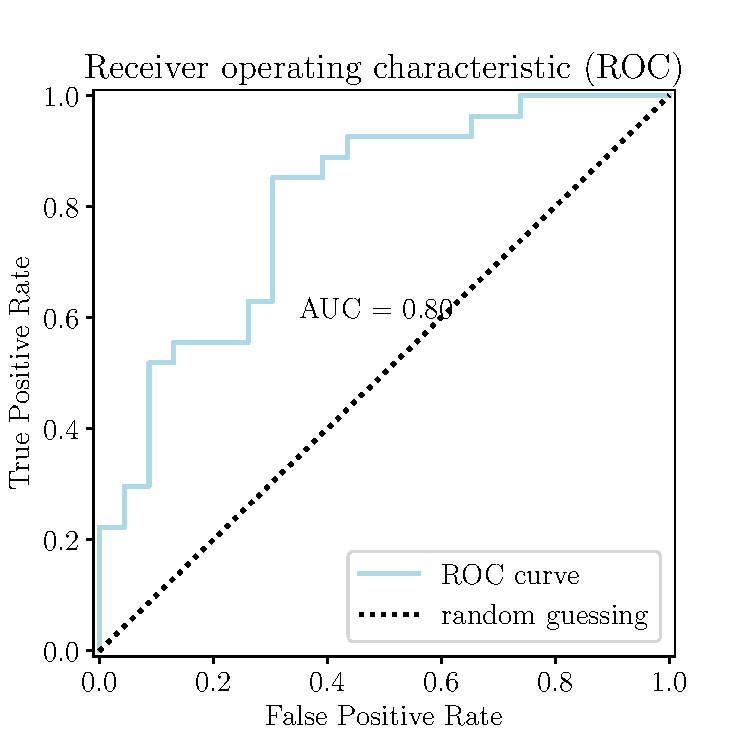
\includegraphics[width=5cm]{ROCplot}
\caption{Example receiver operating characteristic (ROC) curves for different setting of the system}
\end{figure}
\end{column}
\end{columns}
\end{frame}



\begin{frame}{Receiver Operating Characteristics}
\begin{figure}
\includegraphics[scale=0.38]{ROCClass.png}
\end{figure}
\end{frame}

\begin{frame}{Summary}
\begin{itemize}
\setlength{\itemsep}{6pt}
\item To minimize the overall risk, choose the action that
minimizes the conditional risk $R(\alpha|{\rm x})$.
\item To minimize the probability of error, choose the class that maximizes the posterior probability $P(\omega_j|{\rm x})$.
\item If there are different penalties for misclassifying patterns
from different classes, the posteriors must be weighted
according to such penalties before taking action.
\item Do not forget that these decisions are the optimal ones under the assumption that the ``true'' values of the
probabilities are known.
\end{itemize}
\end{frame}

\section{BDT-Discrete}
\subsection{}
\begin{frame}{}
\begin{variableblock}{\centering \Large \textbf{\vspace{4pt}\newline Bayes Decision Theory - Discrete Features\vspace{4pt}}}{bg=slidecolor,fg=white}{bg=slidecolor,fg=white}
\end{variableblock}
\end{frame}

\begin{frame}{Bayes Decision Theory - Discrete Features}
\begin{itemize}
\item Components of ${\rm x}$ are binary or integer valued, ${\rm x}$ can take only one of $m$ discrete values ${\rm v}_1,{\rm v}_2,\ldots,{\rm v}_m$
\item Case of independent binary features in 2 category problem\\
Let ${\rm x}=[x_1,x_2,\ldots,x_d]^t$ where each $x_i$ is either 0 or 1, with probabilities:

~~~~~~~~~~~~$p_i=P(x_i=1|\omega_1)$\\
~~~~~~~~~~~~$q_i=P(x_i=1|\omega_2)$\\
$p_i>q_i\Rightarrow x_i$ is more likely to have value 1 if ${\rm x}\in \omega_1$
\item Class conditional probabilities
\[\boxed{p({\rm x}|{\omega _1}) = \prod\limits_{i = 1}^d {p_i^{{x_i}}{{\left( {1 - {p_i}} \right)}^{1 - {x_i}}}}} ~~~~~~\boxed{p({\rm x}|{\omega _2}) = \prod\limits_{i = 1}^d {q_i^{{x_i}}{{\left( {1 - {q_i}} \right)}^{1 - {x_i}}}} }\]
\end{itemize}
\end{frame}

\begin{frame}{Bayes Decision Theory - Discrete Features}
\begin{itemize}
\item Then the likelihood ratio is given by
\[\frac{{p({\rm x}|{\omega _1})}}{{p({\rm x}|{\omega _2})}} = \prod\limits_{i = 1}^d {{{\left( {\frac{{{p_i}}}{{{q_i}}}} \right)}^{{x_i}}}{{\left( {\frac{{1 - {p_i}}}{{1 - {q_i}}}} \right)}^{1 - {x_i}}}} \]
\item we know that
\begin{figure}
\includegraphics[scale=1]{DB03a}
\end{figure}
\item Therefore discriminant function will be
\begin{figure}
\includegraphics[scale=1]{BayesD05}
\end{figure}
\end{itemize}
\end{frame}


\begin{frame}{Bayes Decision Theory - Discrete Features}
\begin{itemize}
\item We note especially that this discrimant function is linear in the $x_i$ and thus we can write
\begin{figure}
\includegraphics[scale=0.95]{Ch0213}
\end{figure}
\item Decide $\omega_1$ if $g({\rm x})>0$ and $\omega_2$ if $g({\rm x})\leq 0$
\end{itemize}
\end{frame}

\begin{frame}{Bayes Decision Theory - Discrete Features}
\begin{itemize}
\item If $p_i=q_i$, $x_i$ gives us no information about the state of nature, and $\omega_0$.
\item If $p_i>q_i$, then $1-p_i<1-q_i$ and $w_i$ is positive. Thus in this case a ``yes'' answer for $x_i$ contribute $w_i$ votes for $\omega_1$.
\item Furthermore, for any fixed $q_i<1$,~$w_i$ gets larger as $p_i$ gets larger.
\item On the other hand, if $p_i<q_i$, $w_i$ is negative and a ``yes'' answer contributes $|w_i|$ votes for $\omega_2$.
\end{itemize}
\end{frame}

\begin{frame}{Example to solve}
\textbf{\color{blue} Question:}\\
\textit{\color{mycolor2}Compute Bayesian decision for three-dimensional binary features}\\
Suppose two categories consist of independent binary features in three dimensions
with known feature probabilities. Let us construct the Bayesian decision boundary if
$P(\omega_1 ) = P(\omega_2 )=0.5$ and the individual components obey:
\begin{equation}
\left\{ {\begin{array}{*{20}{c}}
{{p_i} = 0.8}\\
{{q_i} = 0.5}
\end{array}} \right.~~~~~~i = 1,2,3\nonumber
\end{equation}
\vspace{2.5cm}
\end{frame}

\begin{frame}{Example to solve}
\textbf{\color{blue} Question:}\\
\textit{\color{mycolor2}Compute Bayesian decision for three-dimensional binary features}\\
Suppose two categories consist of independent binary features in three dimensions
with known feature probabilities. Let us construct the Bayesian decision boundary if
$P(\omega_1 ) = P(\omega_2 )=0.5$ and the individual components obey:
\begin{equation}
\left\{ {\begin{array}{*{20}{c}}
{{p_1} = {p_2}=0.8},~p_3=0.5\\
{{q_1} = {q_2} = {q_3} = 0.5}
\end{array}} \right.\nonumber
\end{equation}
\vspace{2.5cm}
\end{frame}


\begin{frame}{Addition Examples:}
\textbf{\color{blue} Question:}\\
\begin{figure}
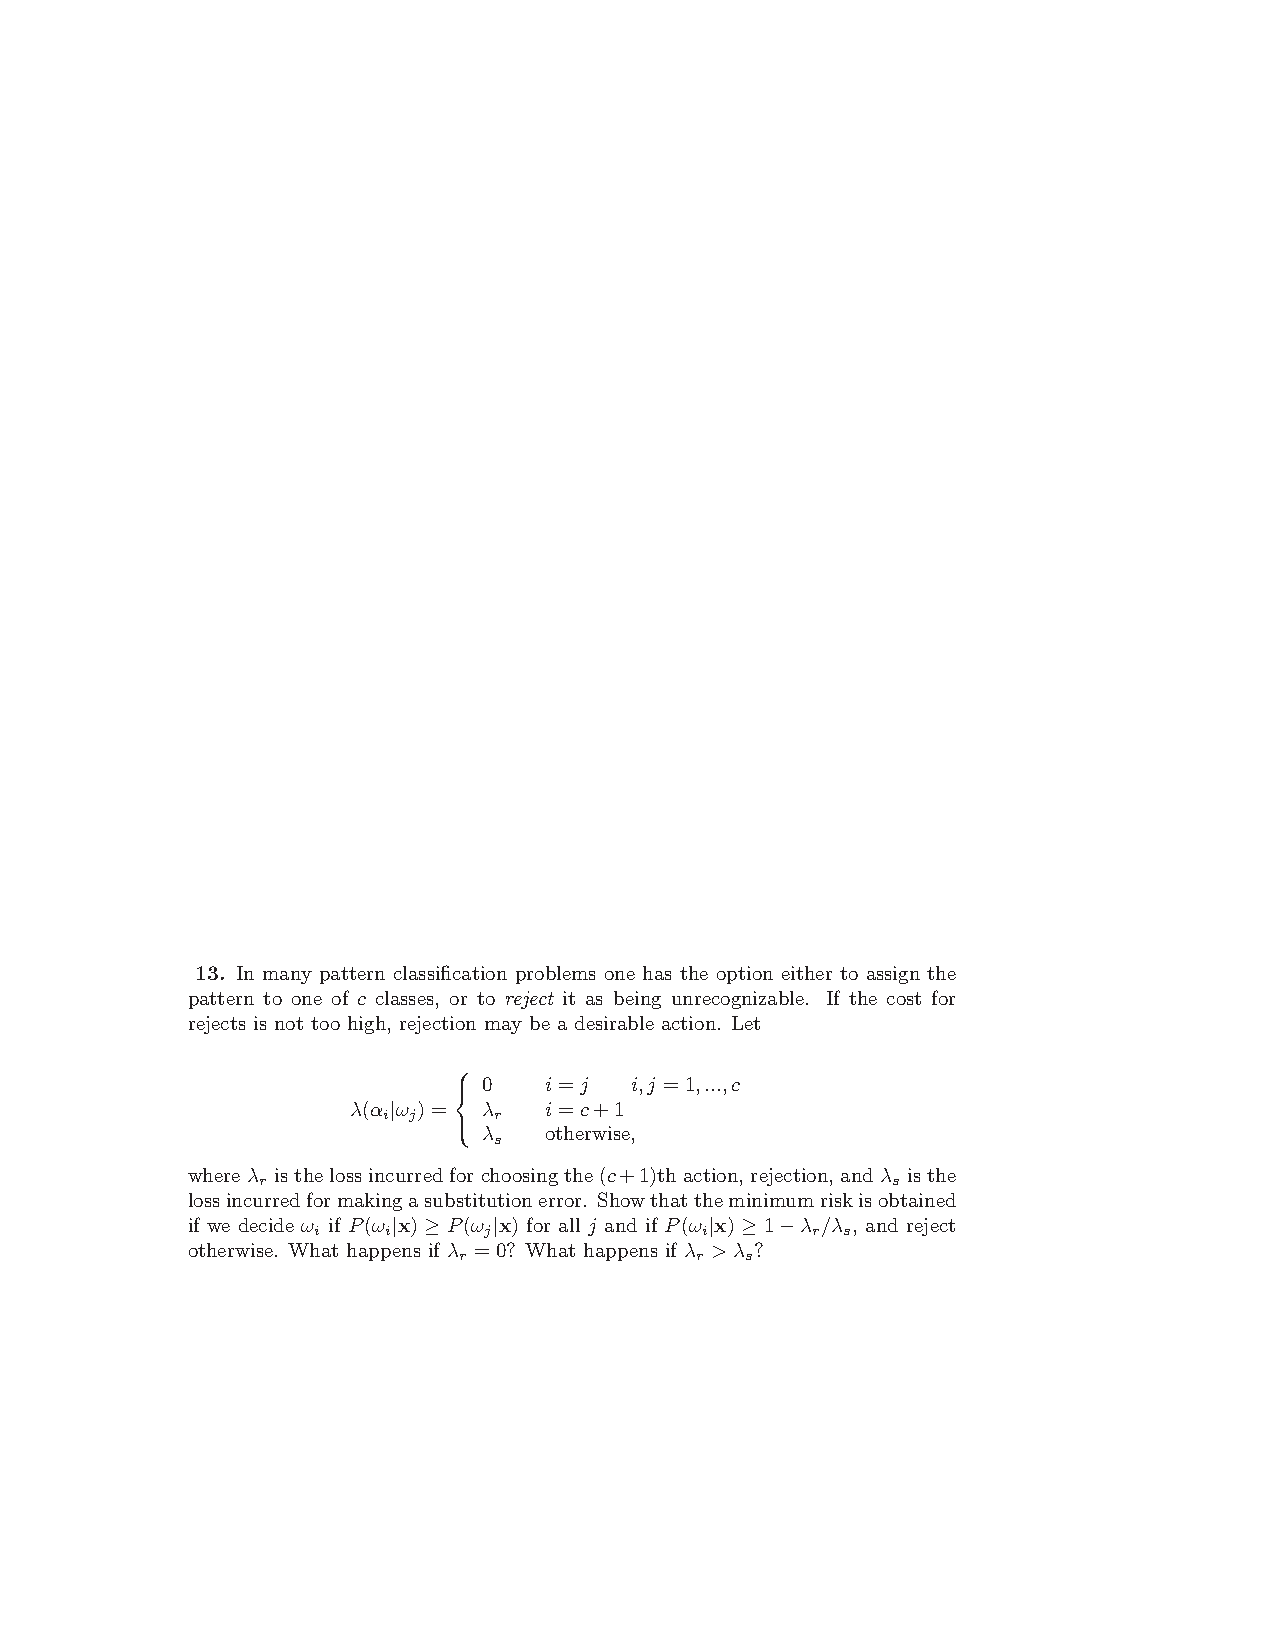
\includegraphics[width=\textwidth]{Question001.pdf}
\end{figure}
\textbf{\color{blue} Question:}\\
What is the inverse of $\left[ {\begin{array}{*{20}{c}}
  4&4 \\ 
  1&2 
\end{array}} \right]$?
 
\end{frame}
\section{References}
\subsection{}
\begin{frame}[allowframebreaks]{References}
\linespread{1}
\footnotesize
\printbibliography[heading=none]
\end{frame}
{
\setbeamertemplate{logo}{}
\makeatletter
\setbeamertemplate{footline}{
        \leavevmode%
  
  % First line.
  \hbox{%
  \begin{beamercolorbox}[wd=.2\paperwidth,ht=\beamer@decolines@lineup,dp=0pt]{}%
  \end{beamercolorbox}%
  \begin{beamercolorbox}[wd=.8\paperwidth,ht=\beamer@decolines@lineup,dp=0pt]{lineup}%
  \end{beamercolorbox}%
  } %
  % Second line.
  \hbox{%
  \begin{beamercolorbox}[wd=\paperwidth,ht=\beamer@decolines@linemid,dp=0pt]{linemid}%
  \end{beamercolorbox}%
  } %
  % Third line.
  \hbox{%
  \begin{beamercolorbox}[wd=.1\paperwidth,ht=\beamer@decolines@linebottom,dp=0pt]{}%
  \end{beamercolorbox}%
  \begin{beamercolorbox}[wd=.9\paperwidth,ht=\beamer@decolines@linebottom,dp=0pt]{linebottom}%
  \end{beamercolorbox}%
  }%
        }
\makeatother

\begin{frame}
\centering
\includegraphics[width=0.4\paperwidth]{queries.jpg}\\
\includegraphics[width=0.5\paperwidth]{thank_you.png}
\end{frame}
}




